\documentclass[9pt,twocolumn,twoside]{../../styles/osajnl}
\usepackage{fancyvrb}
\journal{i524} 

\title{Weather Data Analysis}

\author[1]{Vishwanath Kodre}
\author[1]{Sabyasachi Roy Choudhury}
\author[1]{Abhijit Thakre}

\affil[1]{School of Informatics and Computing, Bloomington, IN 47408, U.S.A.}

\affil[1]{Corresponding authors: sabyasachi087@gmail.com, vkodre@gmail.com, athakre@gmail.com}

\dates{project-000, \today}

\ociscodes{Cloud, I524}

% replace this with your url in github/gitlab
\doi{\url{https://github.com/cloudmesh/classes/blob/master/docs/source/format/report/report.pdf}}


\begin{abstract}
The project aims to analyze any relationship between change in climate, geo- magnetic field and natural disasters with focusing on use of Hadoop Framework for data analysis and Ansible for automating deployment and monitoring.
\newline
\end{abstract}

\setboolean{displaycopyright}{true}

\begin{document}

\maketitle

\section{Introduction}

The study of environmental science and climatic changes around has been done for decades, the study
has always been predictive based on the past experiences and forecasting of the weather conditions
around us. With use of modern days technologies it determining the climatic changes and with analysis
done around it has helped human being to prepare and face the natural calamities. Though with current
equipment weather department has strengthen their arms but has not been able to be full proof and
many time its not been able to predict/ forecast the climatic changes effectively. The study of the
whether data and geo graphical changes is ongoing evolving process. Thus more and more researcher
needs modern days tools and technologies to leverage it and forecast more accurately.

\subsection{Objective}

The goal of this is to study the weather data and analyze the relationship between the geo graphical
changes such change in geo magnetic field and/or natural disaster. With use of Hadoop for distributed
data analysis aims to finds any pattern that might exists between these parameters. The course of the
analysis will also provides visualization of these parameters in order to identify any pattern in a more
intuitive way. By leveraging the power ansible for application deployment over cluster and monitoring
the application performance to determine scalability and throughput. The conclusion will be determine
by establishing any existing pattern, analysis done over it and by visualizing it.

\section{Data Sources}

Weather data has been recorded since 19th century. This data can be used to estimate climate changes
and forecasting. The same data can be can be used to find any existing pattern with natural disasters.
Following sources has been compiled for weather, natural disaster and geo magnetic fields.
\begin{itemize}
\item Weather-Data\cite{Weather-Data}
\item Natural Disaster\cite{Disaster-List-Data}
\item Geo Magnetic Field\cite{Geo-Magnetic-Data}
\end{itemize}

\section{High Level Design}

The design of the application is thought of leveraging power of Hadoop as main processing unit of
analysis with deployment on the cluster environment where application requires multiple processing
units for execution, database for persistence and visualization tools for graphical outputs.
\begin{figure}[htbp]
\centering
\fbox{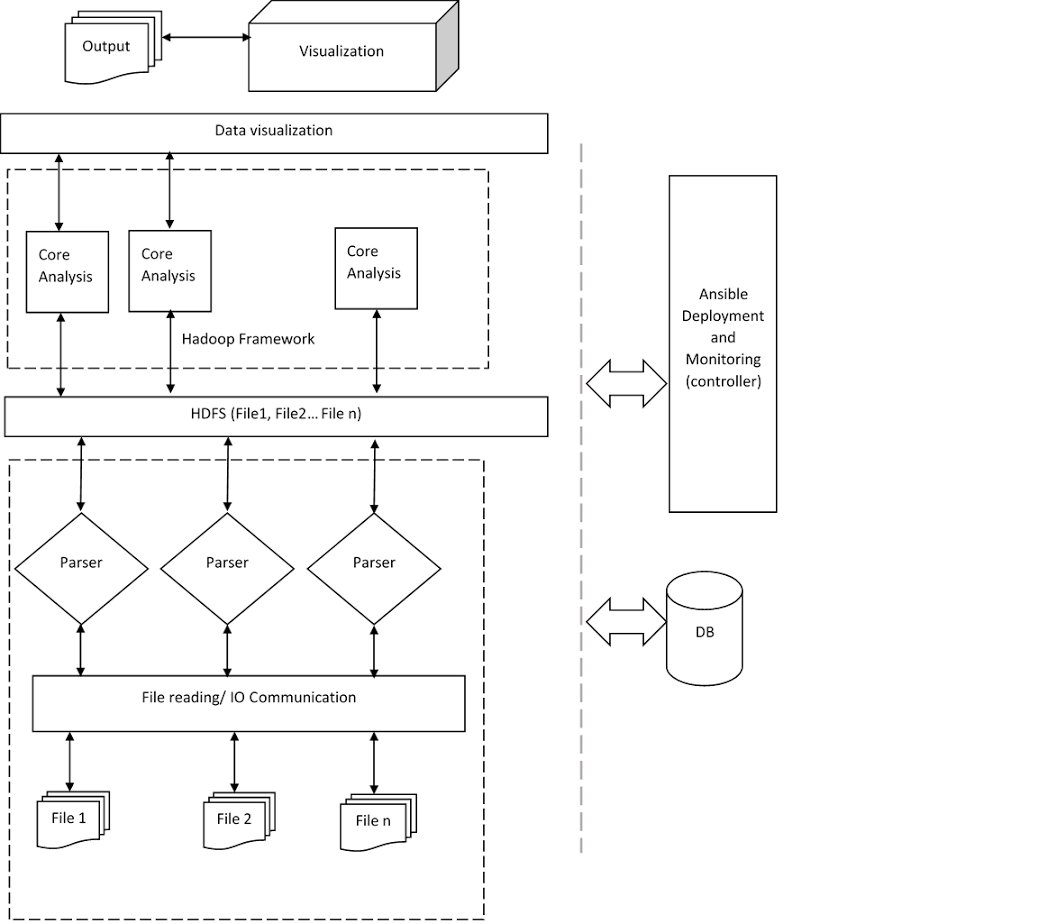
\includegraphics[width=\linewidth]{images/weather_analysis_architecture}}
\caption{Architecture}
\label{Reference:false-color}
\end{figure}
The project is divided into following steps:

\begin{itemize}
\item Data cleaning and persistence - The raw data cannot be use directly for analysis. First data has to be parsed and required parameters will be extracted. Then this extracted data will be dumped into a NoSql database.
\item Core Analysis Program - Core analysis program will be responsible for figuring out any hidden patterns between aforesaid parameters. Program will compare natural disasters occurred, geo-magnetic orientation and climate data
set on a given location and duration and compute relationship between them. The program will be an
MapReduce implementation and is the heart of the application. The program will be executed through
Hadoop framework. Hadoop will execute the program in a distributed manner.
\item Deployment and Monitoring - The application needs multiple processing units and monitoring system. Ansible will be used for deployment and manage nodes for program execution.Ansible will be responsible for following tasks
i)   Deployment and configuration of Hadoop on the multiple nodes.
ii)  Starting Hadoop servers, inserting/reading data.
iii) Execution of the commands to run the analysis using Hadoop to filter the input data and write
response to HDFS or some output file.
iv)  This output can be then passes to the visualization step as the input data.
\item Visualization - Finally once the programs completes execution, using the scikit-tool or other visualization tool
kit and the output file, graphs and patterns depicting the relationship can be plotted more intuitive representation.
\item BenchMarking - The application can be benchmarked for the scalability by addition more nodes and checking the
performance for strong scaling. The report will be represented in tabular format.
\end{itemize}


% Bibliography

\bibliography{references}
 


\end{document}
